\cleardoublepage
\chapter{Implementation and Evaluation}
\label{chapter:evaluation}

We implement an evaluation that attempts to explore the overhead of fastPSI's stronger consistency semantics compared to the weakest Read Committed model, and show how fastPSI is able to outperform a protocol implementing the stronger Serialisability consistency model. We also evaluate fastPSI's scalability as more servers and partitions are added to the system, and discuss some of the weak points of the protocol\todonote{rephrase?}.

\section{Implementation}

Our implementation of the fastPSI protocol consists of a client-side library~\citep{pvc-client} and a server~\citep{pvc-server}, written as a plug-in transactional protocol for Antidote~\citep{antidote-db}, a reference platform for evaluating consistency protocols. Both the client library and the server were written in the Erlang programming language, with a total of 6K lines of code. The Antidote platform provides a key-value database, supports both in-memory and disk-based storage, and implements full replication. For simplicity, our implementation only supports in-memory storage, and lacks a replication mechanism. During normal operation, the client-side library communicates with the server using Google's Protocol Buffers~\citep{protobuf}. To enhance network efficiency, client messages are transmitted in periodic batches to the servers.

To validate the results of our evaluation, we also implemented two alternative protocols satisfying the Read Committed and Serialisability consistency models, called \textbf{naiveRC} and \textbf{naiveSER}, respectively. Both were implemented on top of our original implementation and are as efficient as possible. The pseudocode for both implementations can be found in Appendix~\ref{appendix:code}.

Given that fastPSI requires the use of multiple versions per object, it becomes necessary to prevent an unbounded growth of the number of versions in both the $\VersionLog$ database and the number of entries in the per-partition $\CommitLog$. We implemented a simple garbage collection mechanism that maintains a fixed number of versions and that regularly prunes the oldest versions from the state of a partition.\todonote{Bench for this? Tradeoff between number of versions and abort rate. We should talk about Blotters's TTL GC in related work.}

\section{Evaluation}

We evaluate the performance of fastPSI using the Yahoo! Cloud Serving Benchmark~\citep{ycsb}, modified to generate transactional workloads~\citep{ardekani_nmsi, ardekani_gdur}. Our implementation of Read Committed is used as a baseline for comparison in order to show the maximum possible performance. Figure~\ref{fig:workload-types} describes the workloads used. All experiments are run on a cluster consisting of six core machines with 3.80~GHz to 4.70~GHz Intel Xeon processors, 32~GB of RAM, and a single 1~Gbps network port. We partition the cluster in up to three different sites, with four server machines and four client machines per site. Thus, there is no shared memory between clients and servers, as if clients were acting as proxies in the same data centre as servers. Since all our machines are located in the same local network, we artificially add latency between sites using the \texttt{tc} Linux command.

In all our benchmarks, the system is loaded with one million random keys and 256-byte values prior to receiving any operations from the clients. Keys are mapped to servers using consistent hashing, with clients being aware of the distribution of keys to servers, and thus can directly address all server machines directly. Each client machine spawns multiple concurrent threads that execute transactions and communicate with servers in a closed-loop manner. For the experiments that involve more than one site, the latency between sites is of 10~ms.

\begin{figure}[h]
\begin{center}
\begin{tabularx}{0.85\linewidth}{ c | c | >{\centering}X | >{\centering}X }
    & \multirow{2}{*}{Key Selection Distribution}
    & \multicolumn{2}{c}{Operations}
\tabularnewline
    & & Read-Only Tran.
    & Update Tran.
\tabularnewline
    \hline
    % A & Zipfian & 4 Reads & 2 Reads, 2 Updates \tabularnewline
    B & Uniform & 4 Reads & 3 Reads, 1 Update \tabularnewline
    C & Uniform & 2 Reads & 1 Read, 1 Update \tabularnewline
    % D & Uniform & 3 Reads & 3 Reads, 1 Update \tabularnewline
\end{tabularx}
\end{center}
\caption{Transactional YCSB Workload Types.}
\label{fig:workload-types}
\end{figure}

\subsection{Performance \& Scalability Limits}

\paragraph{Performance.} We begin by investigating the overall performance profile of our implementations by measuring and comparing the throughput and latency of the different protocols as the number of update transactions increases while keeping the number of sites stays constant. For this experiment, we vary the number of concurrent client threads until we reach the saturation point of the system: the maximum throughput it can handle without degrading overall latency in a significant manner. We aim to explore the overall overhead of fastPSI in comparison with naiveRC, and the performance benefits it offers in comparison with naiveSER. To this aim, we use Workload C and three sites. Figure~\ref{fig:general_bench} shows our results. We vary the ratio of read-only to update transactions, from 90\%/10\% to 70\%/30\% (left to right), and measure the termination latency of update transactions, i.e., the amount of time spent on the validation process of a transaction. Since the latency is measured in the client, it only reflects the amount of time spent on the \emph{prepare} phase of the commit validation, as the client does not need to wait until the changes of a transaction are committed to the partition state.

\begin{figure}[t]
\vspace{-0.5cm}
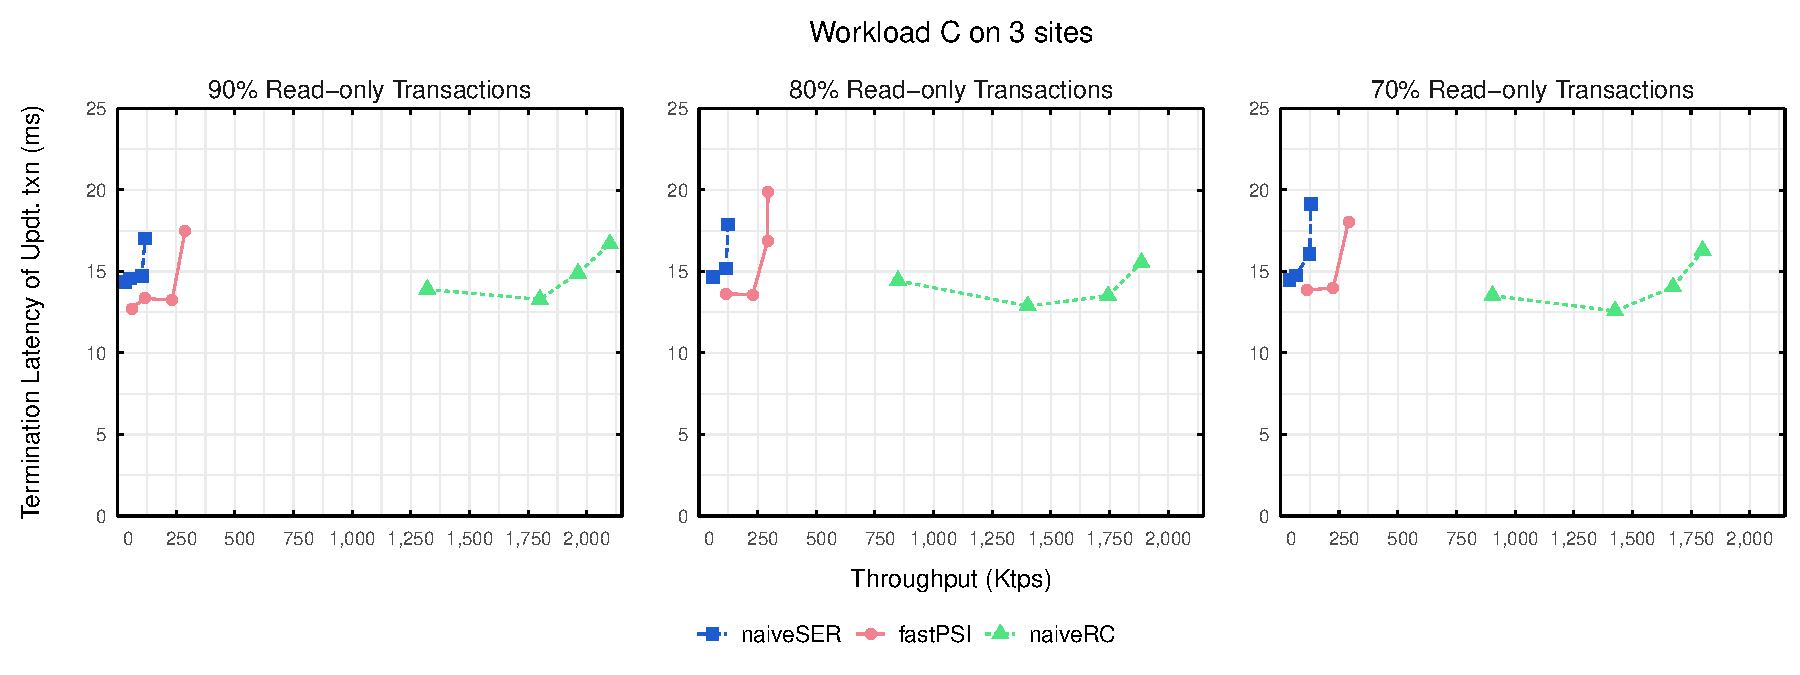
\includegraphics[width=\textwidth]{figures/general_bench.pdf}
\vspace{-1cm}
\caption{Comparison of throughput and termination latency of update transactions.}
\label{fig:general_bench}
\end{figure}

The naiveRC implementation uses 2PC to guarantee atomicity of update transactions, but otherwise proceeds without any validation. Although this is reflected in its high performance, the validation of transactions becomes the only bottleneck of the system, which explains why the overall throughput drops by as much as 20\% as the proportion of update transactions reaches 30\%.

The naiveSER implementation is limited by its need to validate every transaction, and thus its overall performance is not hurt by varying the amount of update transactions. Although fastPSI also exhibits stable performance even as the proportion of update transactions grows, its relaxed consistency model allows it to outperform naiveSER in all cases, by approximately 150\%, while showing similar latencies. However, the overall performance of fastPSI is still limited, having approximately 85\% lower throughput as naiveRC.

% \paragraph{Scalability.} To explore the overall scalability of fastPSI, we

\begin{figure}[h]
\begin{center}
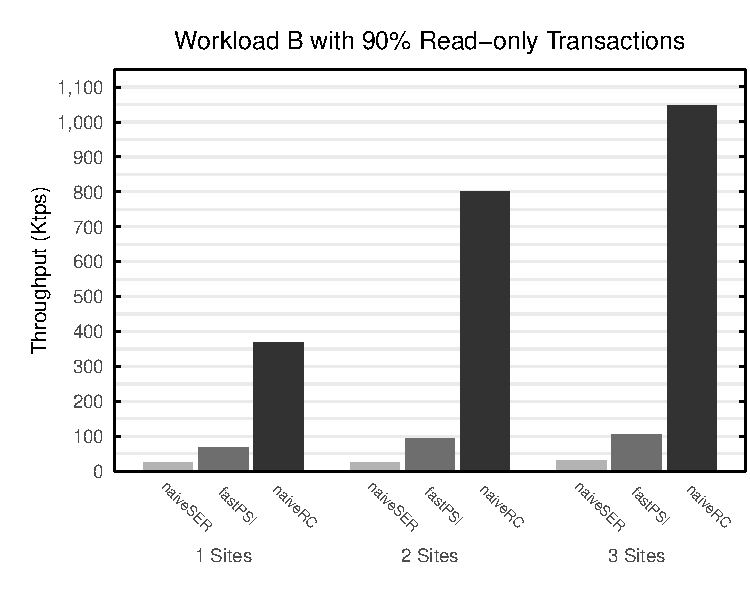
\includegraphics[width=0.5\textwidth]{figures/sites_bench.pdf}
\vspace{-1cm}
\end{center}
\caption{Maximum Throughput of Consistency Models.}
\label{fig:site_bench}
\end{figure}

\begin{figure}[htb!]
\begin{center}
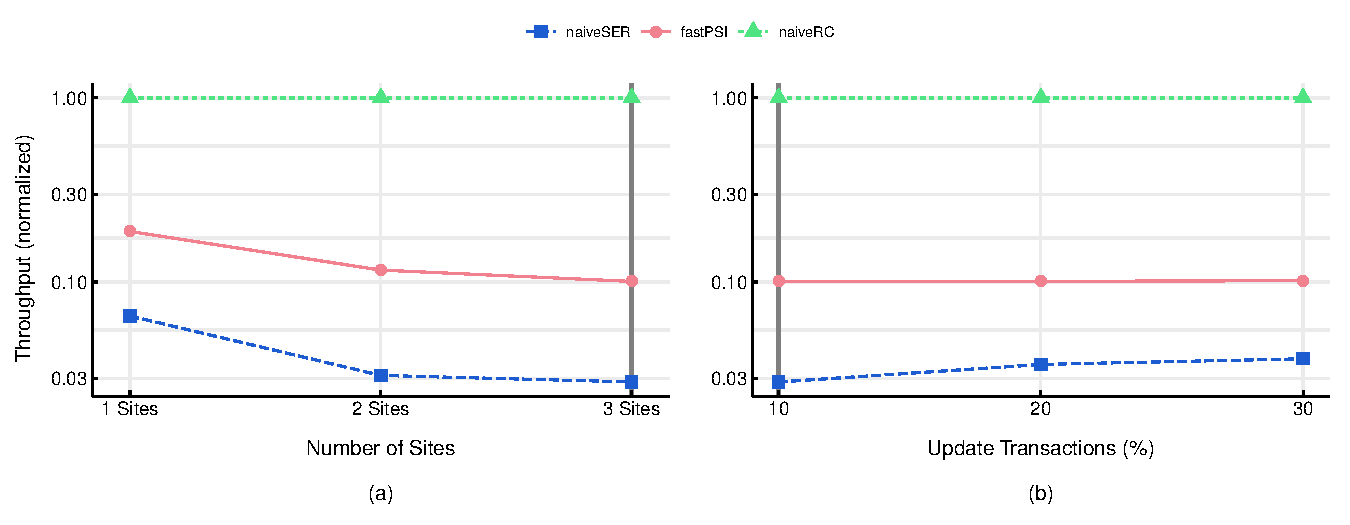
\includegraphics[width=0.6\textwidth]{figures/dynamic_bench.pdf}
\vspace{-0.5cm}
\end{center}
\caption{Some text here.}
\label{fig:dynamic_bench}
\end{figure}

\subsection{Dynamic Workloads}

We now explore the impact of several deployment parameters on the scalability of fastPSI, as depicted in Figure~\ref{fig:dynamic_parameters}.

\begin{figure}[h]
\begin{center}
\begin{tabularx}{0.75\linewidth}{ l | >{\centering}p{5cm} | >{\centering}X }
   \textbf{Parameter} &\textbf{Range} &\textbf{Default}
\tabularnewline
    \hline
    Sites & 1--3 & 3
\tabularnewline
    Update Tran. Proportion & 10\%--30\% & 10\%
\tabularnewline
\end{tabularx}
\end{center}
\caption{Dynamic Workload generator parameters.}
\label{fig:dynamic_parameters}
\end{figure}

\subsection{Read Abort Rate Impact}

\todo{Do we want to compare against SER, or just show combinations that make fastPSI abort more or less? I guess we should so fastPSI against SER in some settings to get a sense of how "good" the abort rate is.}
